\documentclass[10pt]{article}
%\usepackage{fullpage}
\usepackage[top=1in,bottom=1in,left=1in,right=1in]{geometry}
\usepackage{courier}
\usepackage{color}
\usepackage{url}
\usepackage{graphicx}
\newcommand{\PROBLEM}[1] {\textbf{\textcolor{red}{#1}}}

\title{Active RDMA}
\author{Chris Fallin, Anshul Madan, Filipe Milit\~{a}o\\ \\
15-712: Advanced Operating Systems \&  Distributed Systems\\
Carnegie Mellon University}
\date{}
\begin{document}

\maketitle

\begin{abstract}
A classic functionality tradeoff exists between client and server in a
distributed system such as a network filesystem. One approach, widely
used, is to define a static API at the server and allow RPCs to this
API from clients. This approach allows the server implementation to be
optimized for these specific operations. An alternate proposal,
RDMA~\cite{thekkath94}, proposes to allow direct remote memory access
in order to reduce latency and increase flexibility by exposing data
structures directly. However, this approach can suffer from a lack of
performance because code is widely separated from the data on which it
operates. In this project, we propose and prototype a middle ground,
\emph{Active RDMA}, that uses code migration to enable data-code
locality while retaining the flexibility of the RDMA approach. We
propose to run the \emph{active code} directly on the NIC, with full
access to host memory. We modify a full-system simulator and use this
infrastructure to build a proof-of-concept network filesystem, and
provide an initial evaluation of the concept.

\end{abstract}

\section{Introduction}

Traditional distributed services have built upon RPC or RPC-like
interfaces at the network level. In these systems, a server exports a
static set of operations, typically at a high level. For example, a
file server allows a client to open a file in one call, and read a
block of data in the next. An alternate paradigm exists: RDMA (Remote
Direct Memory Access), first proposed in~\cite{thekkath94}, exposes
data structures in the server's memory directly. Client applications
can then, with knowledge of the appropriate structures, implement most
intelligence on the client side and access shared data remotely. The
advantage of this scheme is that it allows low-latency operation if
the RDMA mechanism is implemented efficiently (i.e., in hardware or at
the low level in a system software trap). It also allows more
flexibility in client operations by allowing a finer granularity than
a static high-level API, although this aspect was not evaluated in the
original proposal. The disadvantage is that, for complex
data-structure manipulations or pathological cases (e.g., a long
linked list in memory), the cost of multiple round-trips over the
network can be extreme compared to performing the computation locally
at the server.

We attempt to retain the benefits of both designs by building a
hybrid. In the spirit of Active Networks~\cite{AN-survey}, we propose
to allow clients to send code to the server to execute directly
against the shared data structures. We call this \textbf{Active
  RDMA}. This functionality will allow for the \emph{flexibility} and
\emph{client-driven intelligence} of RDMA while providing the
\emph{data locality} advantages of traditional server-side code.

In order to narrow the scope of our project, we focus specifically on
environments in which security is not an explicit concern. This seems
strange at first in the context of a network-centric project, but
such environments do exist. For example, large computing clusters or
datacenters with a single owner, in which all machines or network
devices are trusted and performance is the paramount concern, are one
possible application domain.

Furthermore, the assumption that security is externally provided
(whole-cluster access control) or otherwise an orthogonal problem
allows us to push Active RDMA's code execution to a lower level,
bypassing layers for higher performance. 

We define our interface to be sufficiently low-level that it could
hypothetically execute directly on a network interface
card~\cite{nic-basedreduction}, interacting with shared memory via
DMA.  This would allow for extremely low latency.

A secondary benefit to this, and one that we explore, lies in the
flexibility of executing arbitrary code segments on the server,
defined by an application. For example, a ``grep''-like operation to
search through some shared data structure might be significantly
faster when executed on the server than when querying a fixed
interface from the client side. (In practice, our ``grep'' was not
optimized enough relative to the system {\tt grep(1)} to show an
actual improvement, but the concept appears sound nonetheless.)

Our work consists of several main contributions:

\begin{itemize} \itemsep -2pt

\item Defining a low-level interface for remote code based on Java
  class-file shipping and both word-level and byte-level shared memory
  access; defining a protocol and building reference implementations
  of a server and a client library to enable use of this Active RDMA
  interface.

\item Building a simulation infrastructure to examine the performance
  tradeoffs of the performance split. We base this infrastructure on a
  conglomeration of the Bochs x86 simulator and the standard Java JVM
  with a timing model, in order to give some level of fidelity
  (however coarse) to our comparison results.

\item Building a distributed file system on top of this
  infrastructure, keeping data in-memory for simplicity, and
  evaluating against NFS; showing use of code shipping to optimize
  \emph{grep} and \emph{find}.

\end{itemize}

\section{Background and Related Work}

As discussed above, the primary advantage of a basic RDMA system is
that there is low latency for common data-transfer operations that
require little actual logic on the server side, and deal with simple
data structures. However, the inability to execute code on the server
can lead to unacceptably high cost for some common operations, such as
a linked list traversal. The proposal in~\cite{thekkath94} gets around
this limitation by also allowing RPC in some cases (e.g., when their
nameserver implementation cannot find an entry after a certain number
of hash-table probes). This is a win for performance, but then
eliminates the flexibility that client-side logic has for
application-specific optimizations. Our Active RDMA idea retains this
flexibility while attempting to regain some of the server-side
performance.

Our work differs in several ways from previous work and other
alternatives:

\begin{itemize} \itemsep -2pt

\item Active Networks are primarily proposed for customization at the
  network or routing layer: for example, upgrading TCP~\cite{AN-tcp},
  or providing programmable packet-forwarding as in ANTS~\cite{ANTS},
  PLANet~\cite{planet} or FIRE~\cite{FIRE}.

\item Active Disks~\cite{AD2,AD} execute code at a disk controller,
  increasing data locality for certain types of data preprocessing in
  the same way as Active RDMA will allow for storage applications.
  However, Active Disks are limited in scope to this data processing.
  In contrast, Active RDMA is a generic mechanism that not only will
  allow for storage applications but any distributed system that
  requires some shared state at a central server. Active RDMA also
  differs in that it proposes to run code directly on the NIC, with
  access to the memory space of the main CPU, enabling more
  interesting and more complex hybrid applications.

\item Mobile code~\cite{mobile} is the name for a general research
  thrust of code migration over networks in order to build distributed
  systems. This is the most similar to our idea. However, mobile code
  is generally a higher-level abstraction that does not provide direct
  access to a shared memory segment, for example, and provides more
  sandboxing and security that removes many of the potential
  performance benefits that we hope to achive.

\end{itemize}

\section{Basic Design}

Active RDMA extends the set of direct memory access primitives --
\emph{read}, \emph{write} and \emph{compare-and-swap} -- to include
two new primitives, \emph{load} and \emph{run}, that load bytecode and
invoke it. The bytecode is executed at the server with access to the
same memory segment that the DMA primitives access, so in theory, the
migration changes only the locality of data access for the shared data
structures.

A representation of this concept is shown in
Figure~\ref{fig:fig1}. The fundamental idea is to move code closer to
data; this allows operations that have longer chains of roundtrips to
be kept local until the final result can be sent back to the client,
at the cost of running code at the server. A simple example is shown
in Figure~\ref{fig:fig2}.

The idea of code shipping is not new, nor is the concept of data
locality. The focus of Active RDMA is to explore how building a
framework that allows clients to make this tradeoff will allow for
more interesting optimizations. The end result might be the same as a
traditional service: code runs on the server locally to compute a
result and return it to the client. The interesting bit is that the
code was sent dynamically by the client, with no prior knowledge from
the server, and it needed to assume nothing about the server other
than its basic interface to a flat memory space.

\begin{figure}
\centering
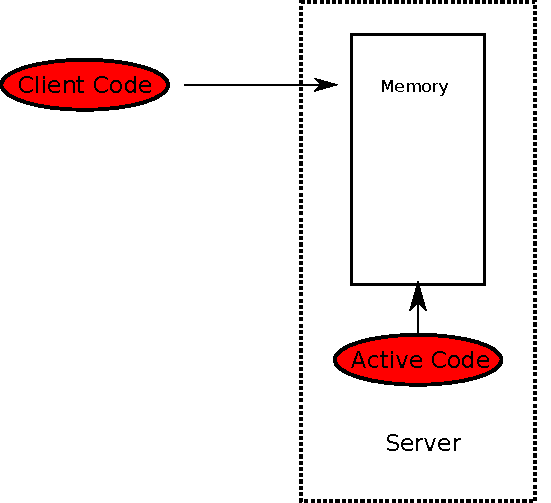
\includegraphics[width=3in]{fig/fig1.pdf}
\caption{Basic Active RDMA code-shipping concept.}
\label{fig:fig1}
\end{figure}

\begin{figure}
\centering
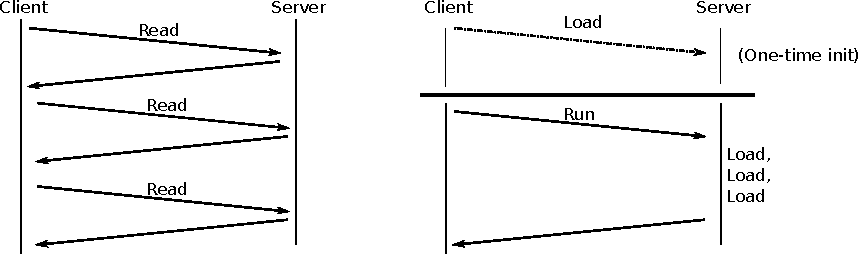
\includegraphics[width=3in]{fig/fig2.pdf}
\caption{Data locality due to code shipping reduces roundtrips.}
\label{fig:fig2}
\end{figure}

\section{Implementation}

We developed a prototype implementation of Active RDMA as a
proof-of-concept and a testbed for initial performance
explorations. We will show here how we develop a fully functional
network filesystem on top of the basic Active RDMA interface.

The most crucial point of our implementation is the definition of the
Active RDMA client-server interface, both at the API level and at the
wire protocol level, since it needs to be simple and small but
powerful enough to facilitate efficient use of the server's
resources. The interface allows direct memory access as well as code
migration (using Java bytecode), and supports the following basic
operations:

\begin{itemize}
  \item {\tt Read}, {\tt Write}, {\tt Compare-and-Swap} -- as in
    original RDMA, these allow for direct memory access over the
    network but both {\tt read} and {\tt write} operations are defined
    over blocks of addresses (so that batching is possible) which
    allows us to group together multiple similar requests in the same
    packet.
  \item {\tt Load(bytecode)} -- loads a Java class file into the
    remote environment. This will cause the class bytecode to be sent
    over the wire and loaded on the server side. The code is then
    indexed using an MD5 hash to detect code duplication and
    disambiguate between multiple version of the same class code
    
    The class is assumed to implement one method, {\tt execute()},
    that takes as parameters a handle to the server memory space and a
    set of arguments passed by the client. The method can return an
    arbitrary chunk of data back to the client. In this way it is as
    general as possible.
    
  \item {\tt Execute(code, param)} -- Executes previously-loaded
    remote code (referenced by MD5 hash), giving it direct access to
    the host memory.
     
\end{itemize}

\subsection{Filesystem}

On top of this basic interface, there is no inherent structure to the
server. Of course, for cooperation to exist between clients in any
reasonable system, some higher-level standard needs to be defined.

We define exactly one system-wide service, {\tt Alloc}, which uses the
first word of the shared segment to point to the next free byte of
memory. This allows clients to use compare-and-swap to atomically
allocate new chunks of memory. (In a real system, of course, we would
implement a full {\tt malloc()} allocator.)

At the next level, we provide a ``root structure'' of sorts by
defining a hash table at the beginning of memory. The hash table
itself is at a known location, and implements linked-list buckets that
are updated atomically by compare-and-swap instructions. This hash
table implements a mapping from arbitrary byte string keys to
pointers. It is up to higher-level applications to assign meaning to
the keys and to the values.

We then begin to build our filesystem-specific infrastructure on top
of this, starting with a simple inode-based datastore. The FS layer
implements arbitrary-length bytestreams, with inode pointers as
handles. Combined with the root hash table, this allows for a flat
datastore.

The final piece of the structure is the high-level hierarchical
filesystem interface. We build ARFS (Active RDMA Filesystem) on top of
the flat-namespace inode store in a very simple way: files are stored
in inodes, with hashtable entries from the full pathname to the inode;
directories are stored likewise, with a special prefix in the key to
indicate that the path is a directory; and directory ``files'' contain
directory entries as in a traditional Unix filesystem. This thin
mapping layer allows performance optimizations at the lower
inode-store layer to propagate upward fairly easily, and it kept
implementation complexity manageable within the scope of this class
project.

The system architecture is depicted in Figure~\ref{fig:fig3}.

\begin{figure}
\centering
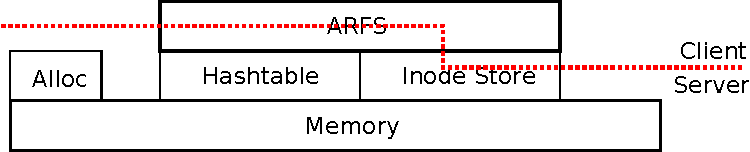
\includegraphics[width=3in]{fig/fig3.pdf}
\caption{ARFS system architecture.}
\label{fig:fig3}
\end{figure}
  
\subsection{System Emulation}

As a final matter, aside from designing the software architecture and
proposing the hardware to run our active code, we must find a way to
evaluate the system. Short of actually constructing or modifying a
network card to run Java bytecode with host memory access, we emulate
the system using a conglomeration of several large pieces of
software. We use Bochs~\cite{bochs}, a full-system x86(-64) emulator,
as our base, and integrate a full Java VM using the JNI (Java Native
Interface) API into the PIC ne2000 network card emulation.

Just as would be required in a real hardware implementation, the NIC
emulation implements a rudimentary UDP/IP stack to talk the Active
RDMA wire protocol. It snoops all packets received by the emulated
system, and intercepts UDP packets destined for port 15712. These
packets are sent to a stripped-down version of our reference platform
server running in the embedded JVM; responses are wrapped in the
appropriate UDP, IP and Ethernet headers and sent, without ever
involving the host system.

The emulated NIC's embedded server has a very simple architecture. It
processes one request at a time, as might be expected from a low-power
processor meant to execute low-latency operations rather than
long-running computations. We also intentionally stuck with UDP rather
than TCP both to maintain statelessness on the server side and to
simplify implementation.

In the proposed system, ultimately, the active code would have access
to host memory and would interact with host software to perform
various functions, if necessary (in the filesystem case, perhaps to
persist data to disk). Since we operated within a limited time budget
and prototyped only the bare minimum functionality, we opted to build
an in-memory filesystem; and since, in this case, no host interaction
is necessary, the embedded JVM is actually completely independent of
the host processor. (We could have allowed it access to host memory,
but then the only ``interaction'' would be allocation of separate
memory blocks from a common pool of RAM, which would serve no purpose
other than possible minimal contention.) Because of this, we actually
implemented an ARP responder in our UDP/IP stack as well, in order to
avoid the need to boot up the emulated Linux system to run pure ARFS
tests. (The common simulator infrastructure is still necessary, of
course, to keep the common network path, timing infrastructure, and so
on.)

Our system emulator architecture is depicted in Figure~\ref{fig:fig4}.

\subsubsection{Timing model}

We collect two forms of timing information with our emulator
infrastructure: \emph{wall-clock time} (as observed by the client) and
\emph{virtual time} (as observed by the server). Since the emulated
components may not run at uniform speed, a completely accurate
evaluation of the system would track virtual time as it progresses
with server events, and produce a synthetic runtime for a given
benchmark. In our emulator, we punt on the very hard problem of
accurately modeling every component at cycle accuracy by simply
tracking various events -- instructions executed on host CPU, network
packets received, memory accesses by the JVM coprocessor, and time
spent in the JVM coprocessor -- in order to come up with a synthetic
runtime from this vector later by assigning costs to each event. In
practice, we found this approach unreliable at best; however, some of
the individual statistics, such as network roundtrips, were useful for
individual evaluations.

\begin{figure}
\centering
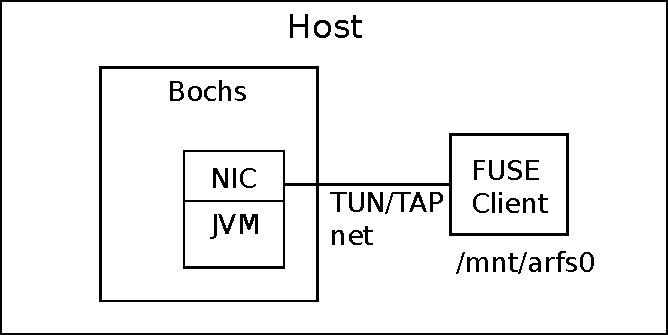
\includegraphics[width=3in]{fig/fig4.pdf}
\caption{Emulator architecture.}
\ref{fig:fig4}
\end{figure}
  
\subsection{Initial demo applications}

We built four simple demo application using our prototype framework. 

\begin{itemize}
\item linked list, designed to maximize dependent pointer chasing and
  thus number of network roundtrips in the non-active case. Insert is
  a naive linear implementation (it traverses the list to find the
  tail), and random fetch is also $O(n)$ as it is for any linked list
  of $n$ elements.
\item hash table, with linked-list buckets.
\item in-memory filesystem (built using the hash table), as described
  previously.
\item locking (mutual exclusion) service with FCFS lock ordering~\cite{nic-basedatomic}.  
\end{itemize}

Running the first two as both plain RDMA and as Active code served as
initial benchmarks whose results encouraged us to continue with the
implementation. The results of running in a local machine (where
network latency and bandwidth should be considerably smaller than any
real remote execution) are shown in Figure \ref{res1}.

\begin{figure}[h!]
\center
\begin{tabular}{|ccc|}
\hline
Algorithm & Operation & Run Time\\
\hline
list - RDMA &  put & 39.675 ms \\
list - RDMA & get & 19.38 ms \\
\hline
list - Active & put & 0.33 ms \\
list - Active & get & 0.245 ms \\
\hline
\hline
table - RDMA  & put & 1.919 ms\\
table - RDMA   & get & 1.739 ms\\
\hline
table - Active  &put & 0.245 ms\\
table - Active & get & 0.239 ms\\
\hline
\end{tabular}
\caption{Results for RDMA and Active operations on a list and hash table.}
\label{res1}
\end{figure}

These results show gains consistent with the complexity of the
operation. Thus, the insertion of 200 elements in a list as well as
the iteration over all those elements has a considerable gain on the
Active version when compared with the RDMA version that requires all
pointer chasing to be serialized over the network. On the hash-table
side, gains were still significant but more modest as this structure
has a lower computational complexity both for insertion and access and
therefore, will pay a lower performance penalty for using the network.

The last two application (the file system and the locking service)
were then extended into the full testing framework discussed further
below.

\subsection{Active RDMA File System Client}

The Active DFS client is implemented as a FUSE file system, which
considerably simplified the development effort over a more traditional
kernel-hosted approach. We used JNI bindings to implement the Active
RDMA client code in Java.

\subsubsection{RDMA and Active variants}

Our filesystem implementation supports mounting in two modes: bare
RDMA, and Active RDMA. In the former mode, all accesses are performed
using only Read, Write and CAS operations; no code migration is
performed. This is implemented as a baseline in order to provide a
comparison point for our ``real''active filesystem.

The Active RDMA filesystem offloads most functionality to server-side
mobile code. Most common filesystem metadata operations, such as file
creation and deletion, happen in one server roundtrip, as would be
expected from a robust network filesystem. The filesystem punts fo the
underlying FS inode-store layer (described above) for the IO path,
which is similarly optimized with active code in order to perform
inode structure traversal and request fragmentation at the server
side. The hashtable lookups are similarly performed by server-resident
active code.

\subsection{DFS utilities (Grep, Copy and Find)}

In order to use the file system and expose our performance gains, we
built the following utilities that make use of the unique
code-migration feature of Active RDMA to access the filesystem at a
higher level on the server side:

\begin{itemize}
\item Copy -- a simple utility that is able to copy a file already in
  the FS to another file. File copy is an obvious application of
  server-resident code, since the data need never traverse the network
  if its final destination is the same filesystem.

\item Grep -- does simple pattern matching on a text file. It takes a
  regular expression that is then used to filter a text file and
  returns all lines that contain that expression. Although we did not
  experiment with more dynamic code generation based on regex
  compilation or other more complex query-driven customizations (that
  would truly expose the advantage of such dynamic system), our
  prototype implementation of this utility should be enough to serve
  as proof-of-concept that our model can achieve significant
  performance gains when compared with purely client side RDMA. Thus,
  we leave as future work the potential to send dynamically generated
  code that matches the data-structures on the server side more
  efficiently, instead of sending the pattern that gets used in a
  generic pattern matcher.

\item Find -- this utility searches for files that match a specific
  name pattern. Like the grep utility described above, it exposes the
  advantage of server-resident code by locally searching the keyspace
  of the hash table for filenames matching a given pattern. As above,
  we compare this find utility to a traditional client-resident RDMA
  implementation of the same functionality.

\end{itemize}

\section{Evaluation}

Finally, having described the system, we will evaluate it both in
absolute terms and in comparison to NFS, hoping to explore some of the
more unique and interesting properties of an Active RDMA-based system.

\subsection{Methodology}

We evaluate three filesystems: NFS, our ARFS mounted as RDMA
(ARFS-rdma), and our ARFS mounted with active code (ARFS-active). All
three are evaluated on our modified Bochs emulation platform, using a
local virtual network (TUN/TAP) from Bochs to the evaluation host
running the network clients.\footnote{The evaluation platform is an
  Intel Core i7 975 Extreme Edition quad-core, with 6 GB of DDR3-1066,
  running 64-bit Ubuntu GNU/Linux 10.04 LTS with kernel 2.6.32-21.}
The host system either mounts ARFS using the FUSE client or NFS using
the standard Linux NFS client.

To make the comparison fair between NFS and the very simple
memory-resident ARFS, we serve the NFS mount off of a RAM disk in the
emulated Linux system. This ensures that disk reads and writes do not
interfere with the measurements. We also manually touch files on the
emulated system before benchmarks on the host system read them, to
ensure that the host system is not caching the files' contents.

The following tests were performed on each filesystem, each 10 times
(to obtain a 95\% confidence interval):

\begin{itemize}
\item Andrew Benchmark~\cite{ab}.
\item Streaming read, using a 5 MB file copied from {\tt /dev/zero}.
\item Streaming write of the same 5 MB file.
\item Find, using the standard {\tt find(1)} utility to find a single source file in the Bochs source tree.
\item Grep, using the standard {\tt grep(1)} utility to find three
  words (apple, zoo, moo) from {\tt /usr/share/dict/words}.
\item Scale, in which the filesystem was mounted at five mountpoints
  concurrently, and an Andrew Benchmark run simultaneously at each
  mountpoint.
\end{itemize}

For each test, we invoked a custom utility to query the server
virtual-time counters immediately before and after the benchmark. We
also recorded the system time (from a high-resolution RT clock) at
both of these points in order to provide wallclock time figures. Our
postprocessing then found the deltas in each counter and constructed
means and confidence intervals, from which we were able to obtain our
final results.

In actuality, we were able to glean far less from the virtual time
counters than we had hoped we would be able to. Originally, we wanted
to construct a virtual time function as a linear combination of the
event counter vectors; it turns out that real systems are much more
complex than this, as some events are off the critical path and others
happen in parallel. We thus resort to presenting wallclock time first,
with the understanding that this is not the most trustworthy
comparison due to the disparity in speed between the emulated host CPU
and the JVM ``coprocessor'' running on the native host. A more
complete evaluation methodology, developed postmortem, is presented in
Future Work below.

\subsection{Results}

We present wallclock time results first in
Figures~\ref{wallclock}~and~\ref{wallclock2}. As mentioned previously,
the disparity in speed between the JVM and the Bochs CPU provides an
artificial advantage to ARFS. Nevertheless, these results are
interesting because (i) they provide some sense of possible client
performance, at least, and (ii) they are better than nothing. The
results also show that ARFS-active is a marked improvement over
ARFS-rdma, as expected.

Figure~\ref{wallclock2}, in particular, shows the rather embarrassing
result that our custom Grep and Find utilities are several times
slower than the respective native Unix utilities running on our
filesystem, even when active code is used (that is, Active-Grep with
active code is still slower than native grep). The most likely
explanation is simply that our utility is naive and unoptimized,
whereas native grep is heavily optimized. Its in-memory data
structures are especially superior for larger-than-trivial files as
compared to our utility's use of the Java class library regex
implementation.

Next, we present CPU load as a function of a scaling client base in
Figure~\ref{cpuload}. This plot compares CPU time in NFS, normalized
to a 2 GHz host CPU running at 1 IPC (instruction per cycle), against
the JVM execution times. We see that the scaling in ARFS is greater
than that in NFS, most certainly due to the push of functionality
toward the server that characterizes ARFS. (Interestingly, ARFS-rdma
also exhibits significant JVM coprocessor load, due to the high
read/write/CAS request density; if these requests were handled
directly in hardware, there would be no coprocessor overhead in the
RDMA case.)

We also evaluated packet roundtrips for each filesystem, with the
results presented in Figure~\ref{rt}. We take two conclusions from
this plot. First, the reduction in roundtrips that Active RDMA enables
over base RDMA is striking: ARFS-rdma exhibits as many as 3x
roundtrips as ARFS-active in these basic filesystem performance
tests. However, ARFS-active still makes use of more packet roundtrips
than NFS. This is due to NFS' request block size and
response-fragmentation behavior: a single roundtrip in NFS can invoke
a response of, for example, 4KB, that is split over multiple UDP
packets because of the Ethernet MTU, whereas an ARFS response is
limited to one packet due to simplistic design.

Finally, we evaluate the impact of reduced roundtrips due to active
code explicitly by deriving a synthetic time function in
Figure~\ref{synth_time} as a function of packet latency. Here we take
the JVM execution time and add the number of roundtrips multiplied by
some RTT latency in order to obtain the synthetic execution time for
the Andrew benchmark (assuming an infinitely fast client). This is
actually a valid approach because there is no parallelism in our
simplistic design: a request packet is sent, the server churns, and a
response is sent; after that arrives, the next request packet can be
sent. So the critical path is a strict sum of each of these
components. The base RDMA runtime (at zero latency) is greater
because, as mentioned above, the coprocessor also handles
read/write/CAS requests; if it did not, this line would be at the
origin for latency zero, but would quickly exceed the runtime for the
active-code system.

\begin{figure}
  \centering
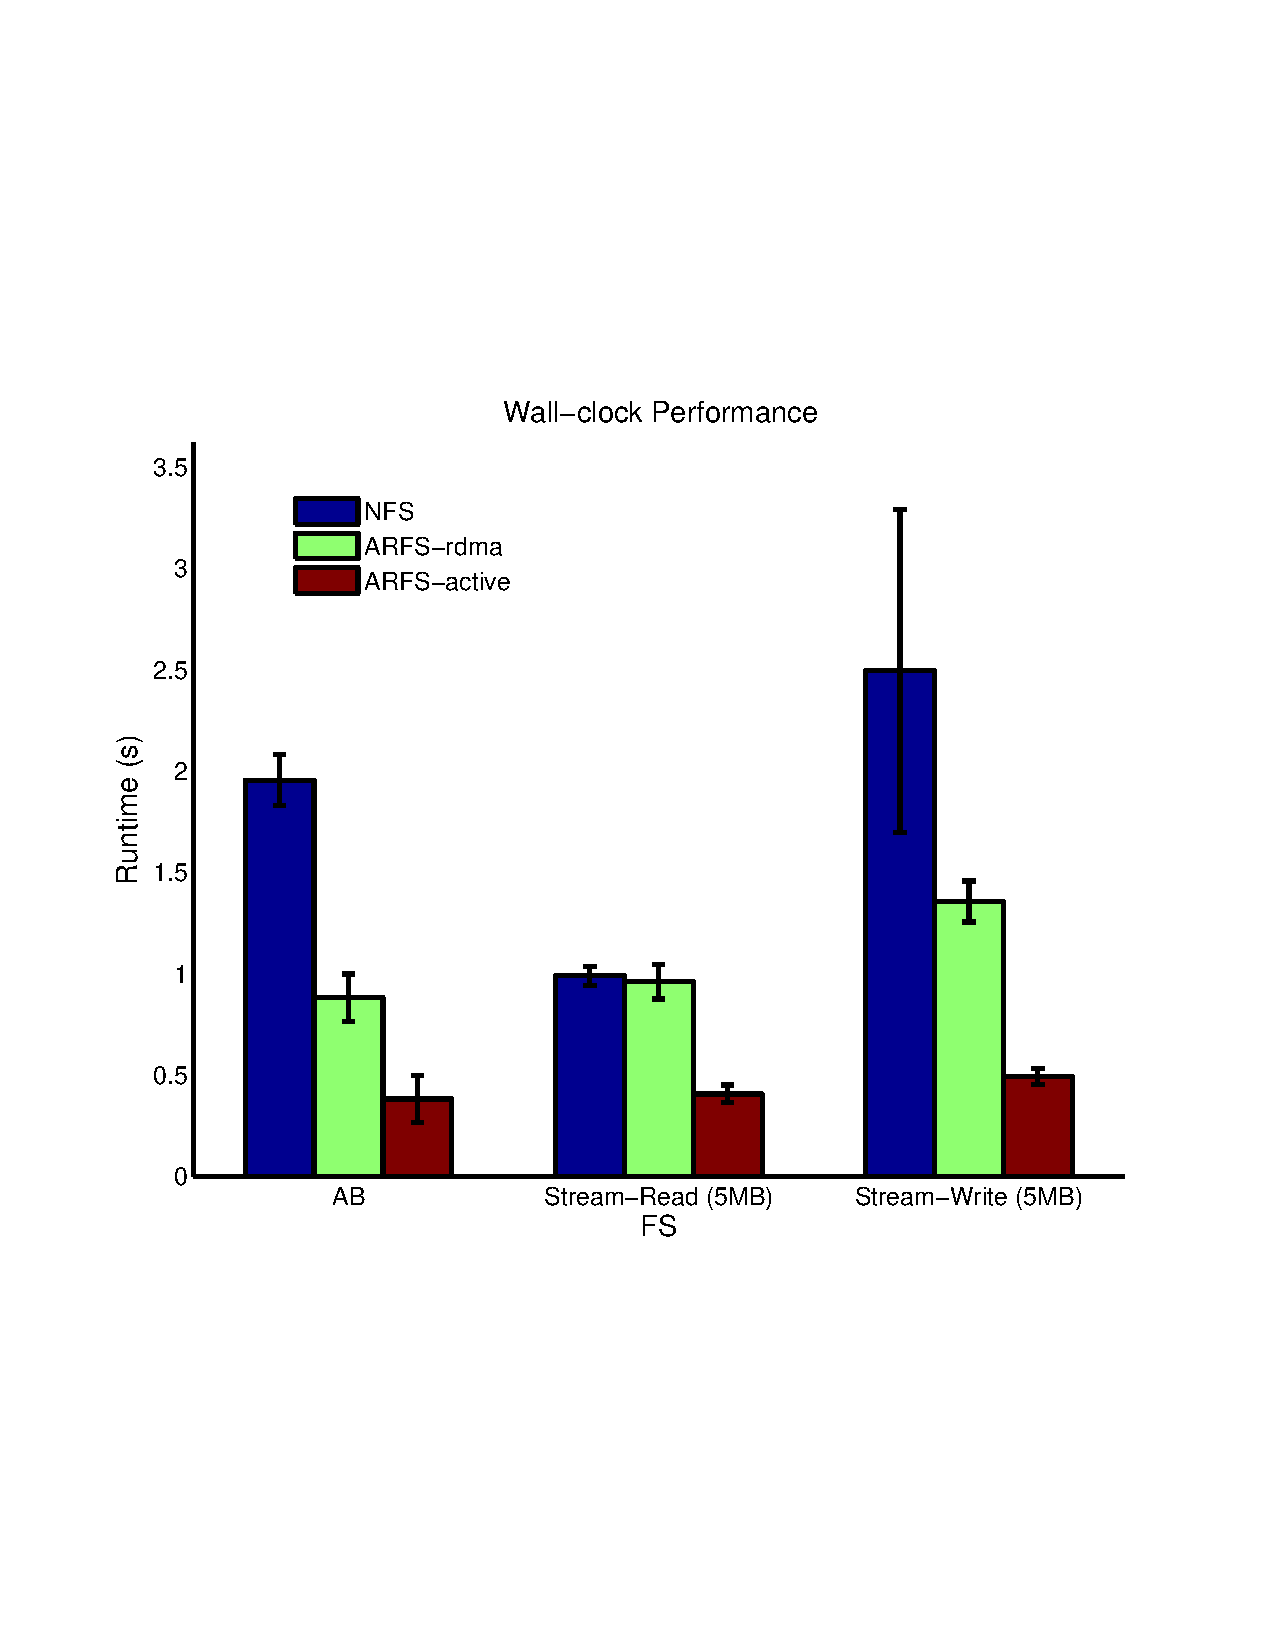
\includegraphics[scale=0.5, trim = 0 200 0 200]{../../results/matlab/wallclock.pdf}
  \caption{wallclock}\label{wallclock}
\end{figure}

\begin{figure}
  \centering
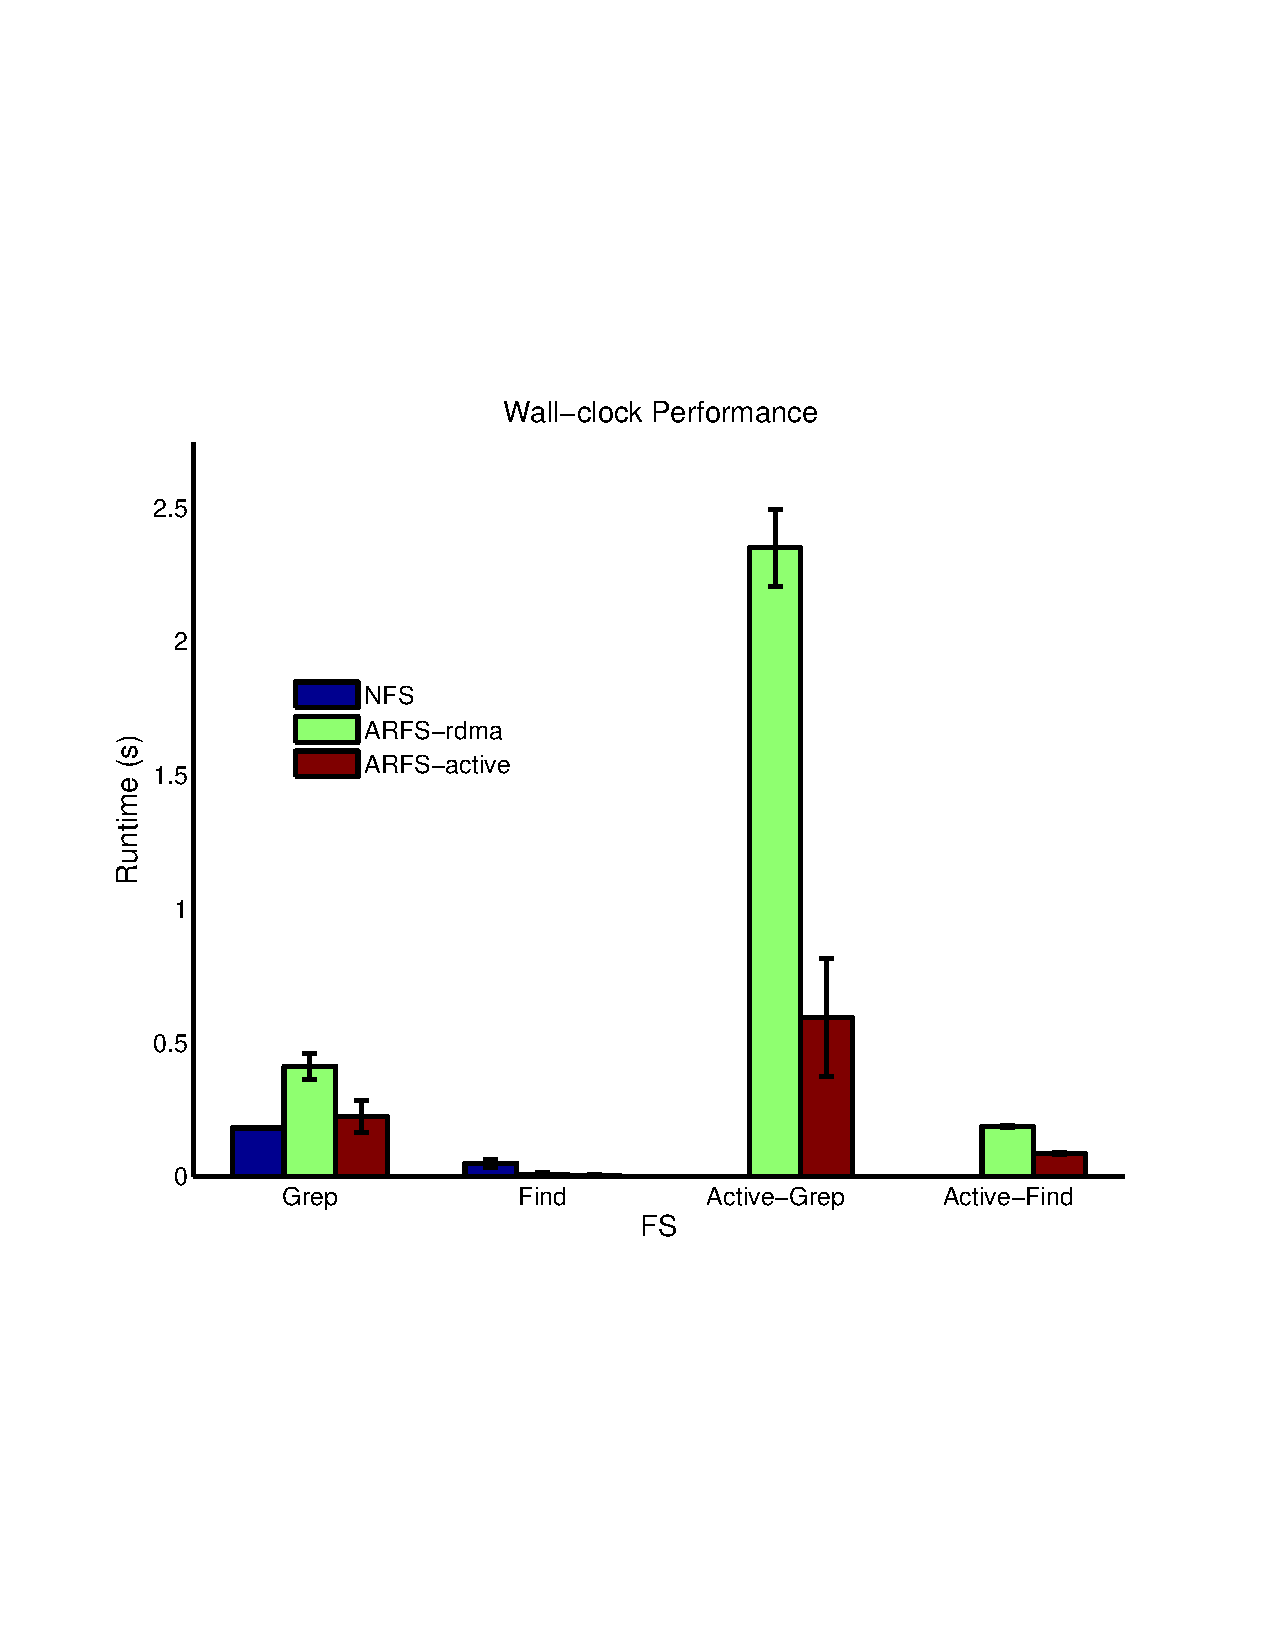
\includegraphics[scale=0.5, trim = 0 200 0 200]{../../results/matlab/wallclock2.pdf}
  \caption{wallclock2}\label{wallclock2}
\end{figure}


\begin{figure}
  \centering
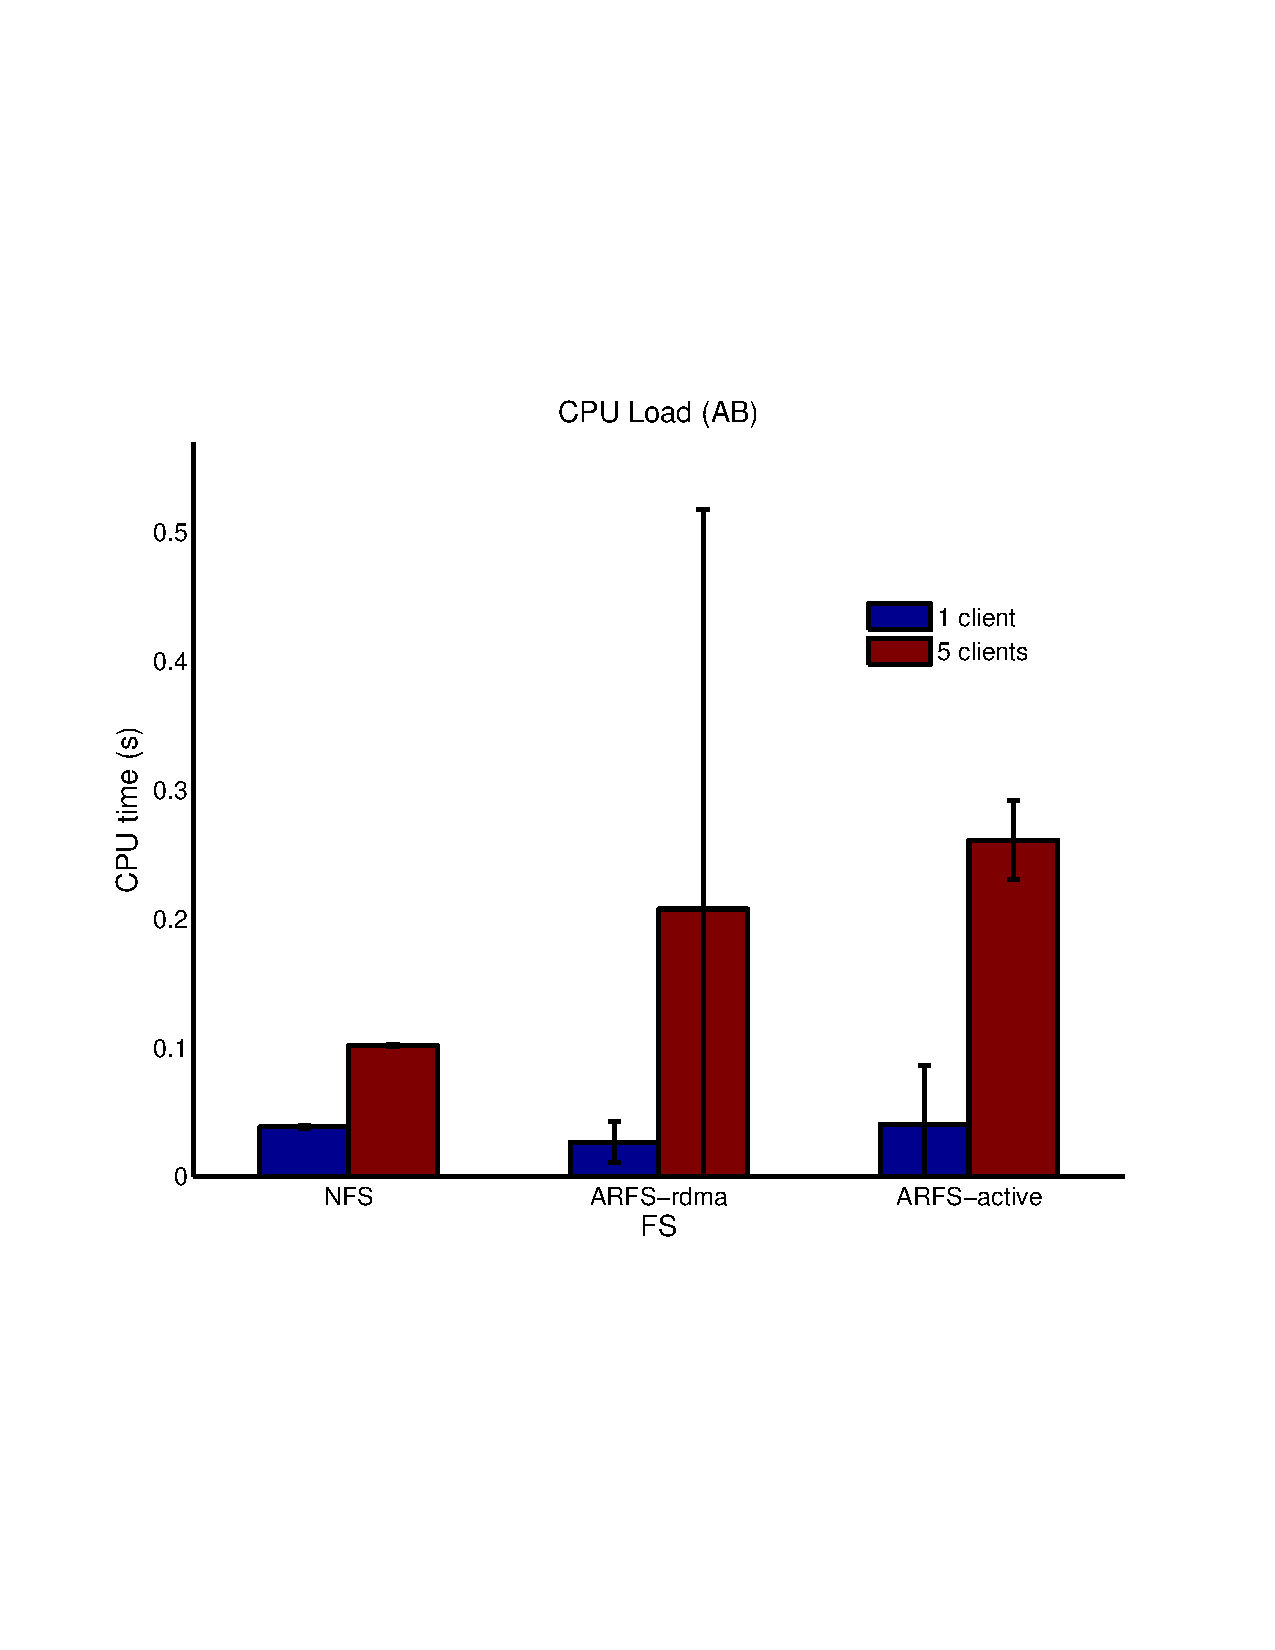
\includegraphics[scale=0.5, trim = 0 200 0 200]{../../results/matlab/cpuload.pdf}
  \caption{cpu load}\label{cpuload}
\end{figure}

\begin{figure}
  \centering
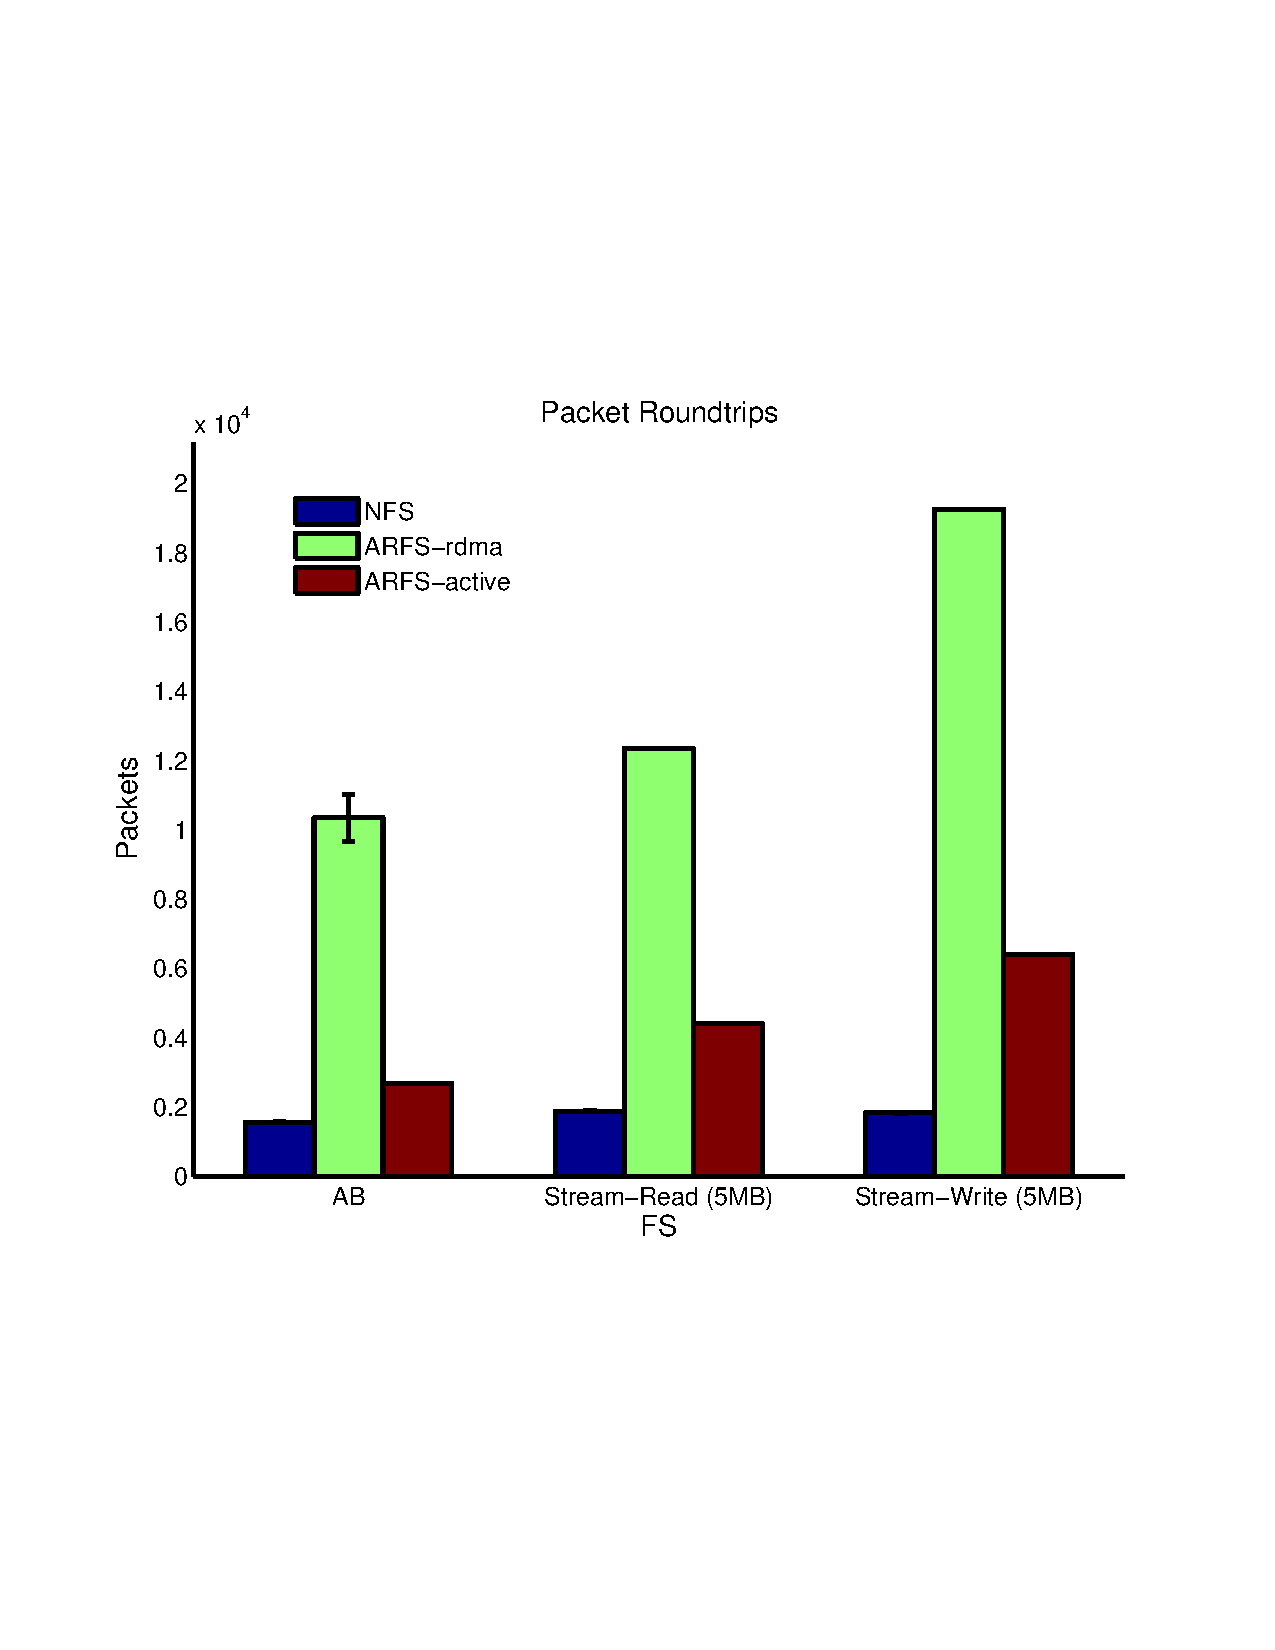
\includegraphics[scale=0.5, trim = 0 200 0 200]{../../results/matlab/rt.pdf}
  \caption{rt}\label{rt}
\end{figure}

\begin{figure}
  \centering
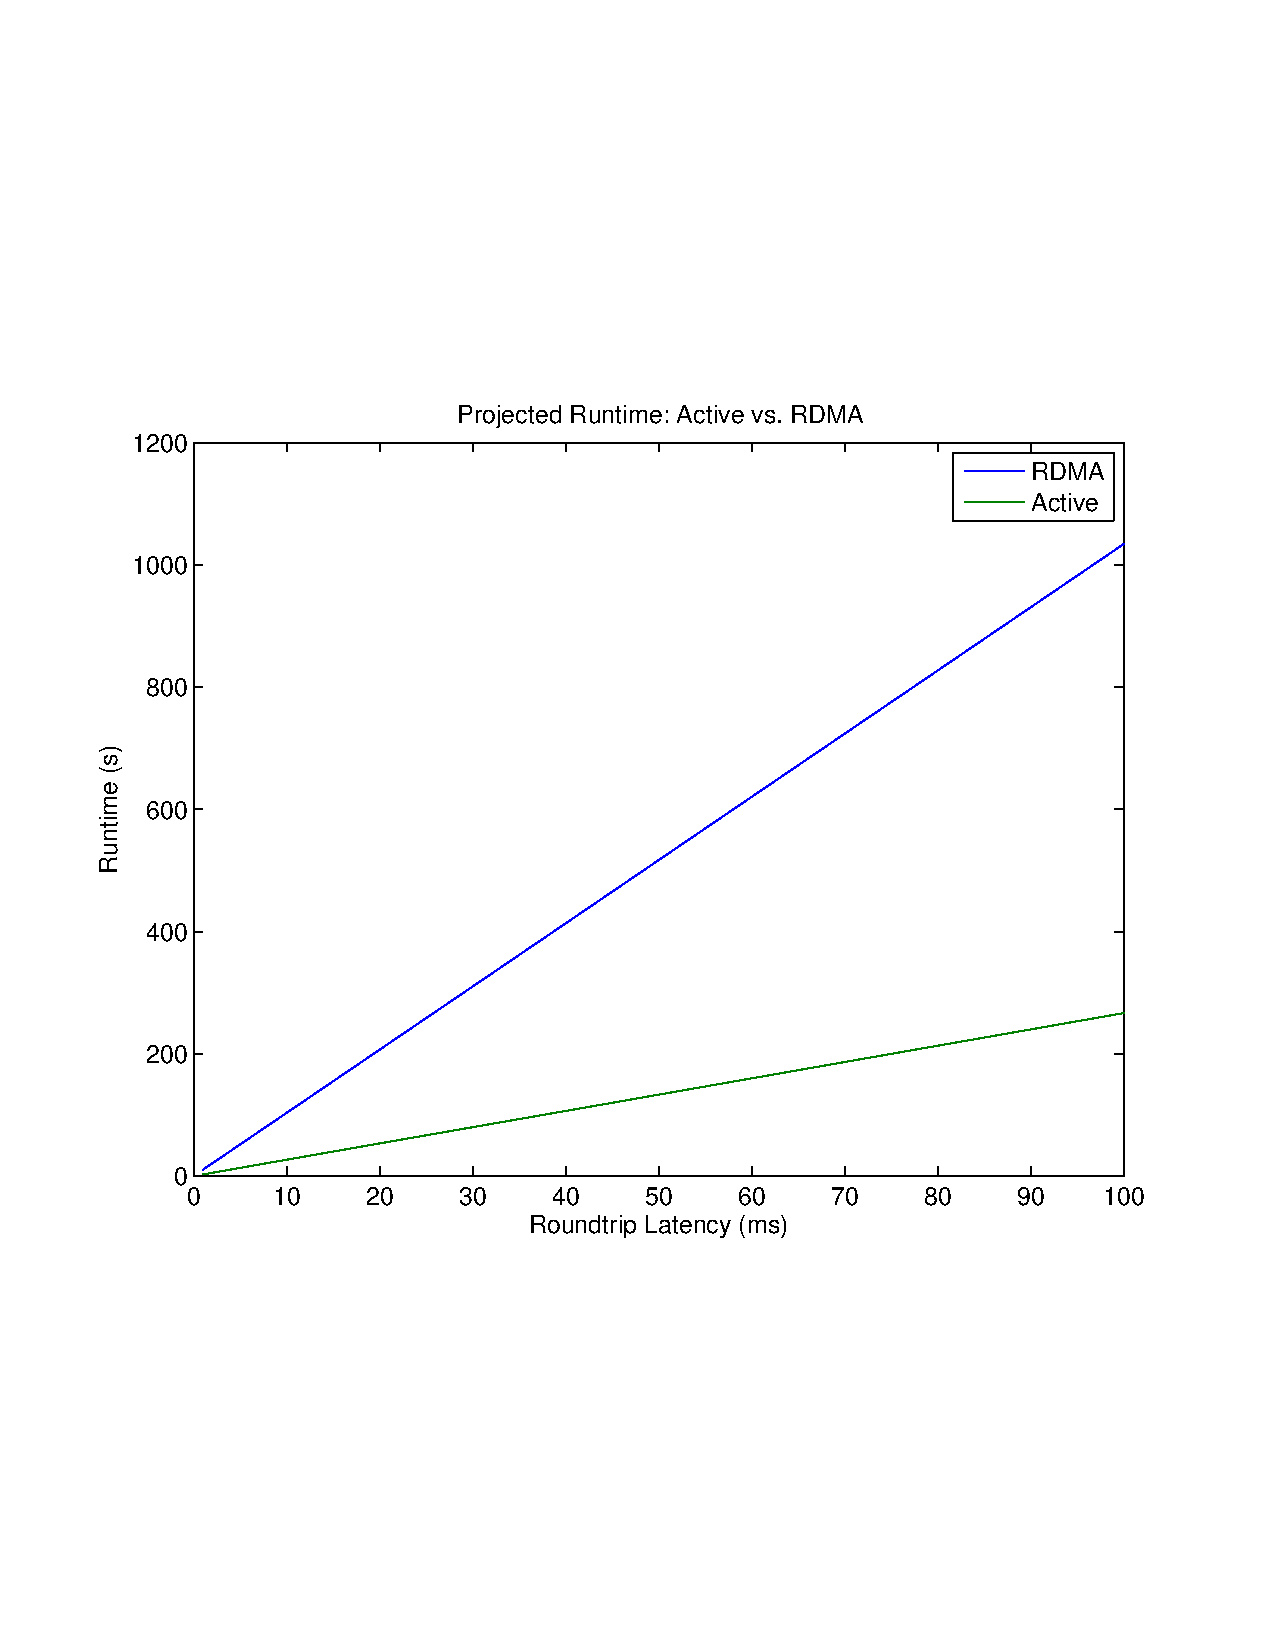
\includegraphics[scale=0.5, trim = 0 200 0 200]{../../results/matlab/synth_time.pdf}
  \caption{synth time}\label{synth_time}
\end{figure}


% ------------------------------------------- cfallin pass head-pointer -------------------------------------------------------------

\section{Future Work}
The fairest way to evaluate would be to have a real system with a real network card
with a real coprocessor running the JVM.

\section{Evaluation Discussion}
The simulator models a main processor running Linux and a coprocessor that
runs the JVM. The JVM is not run on the simulated Linux system, because
it would be terribly slow it would still not be a fair comparison, since
the actual Active RDMA code would run on the NIC card. The fairest
way to evaluate would be to have a real system with a real network card
with a real coprocessor running the JVM, but that is part of future work


Basically, for NFS the overall protocol processing overhead needs to be
taken into consideration, the NFS server has stats that can help
in calculating the execution times things like counts and times of
nfs\_getattr, nfs\_stat, nfs\_read are maintained by Linux NFS servers. These
would include the overall execution time for different nfs operations. But 
we would still not be able to compare these results against the Active ARFS
and ARFS RDMA because of the different processor speeds.

Another way to compare NFS against Active ARFS would be for us to collect
'CPU load' plot which counts instructions against the stats like
time spent in the JVM(coprocessor) that we collect. Though that still
does not give a fair comparison because it does not take into consideration
the difference in processor speeds.

What is most important in the comparison of NFS against ARFS is the total
time between when the client sends the DFS request and when it receives the
reply. Thus packet latencies alone are not that important , but number of packet
roundtrips compared for NFS compared( and contribution of each packet to the
overall execution time ) to the same test run on ARFS is more important. So
as the packet latencies increase, ARFS would perform better than NFS because
it has lesser number of roundtrips.

Our performance measurements have the number of roundtrips(pkts), and we have
the execution time for ARFS(jvm\_nsec), so if we get NFS execution time from
our stats, then we could compare the execution times as well as the total time
from when the packet leaves the client to when the client gets back the reply.
We get total time by assigning latencies to the each paket (= latency * packets).

Since jvm\_nsec is a diff taken at start and stop of processing at the JVM coprocessor,
then memory access times are already included in jvm\_nsec. So we should not include mem\_* for
calculating execution time.

To get a fair comparison we would require a complete real system, or else full-system emulation of
server and all clients in a synchronized time domain with realistic JVM speeds.

To compare Avtive ARFS vs RDMA ARFS we use a Synthetic Time approach.

Since we are simulating different things at different speeds, we use the "synthetic time"
approach , wherein we're measuring the different components that contribute to time directly
and then taking a linear combination of them to get a synthetic (simulated) execution time.

To simulate different memory access times, we have the number of ARFS memory accesses like
r(), w(), cas() and these can be sweeped ro detrmine execution time. We can assume a reasonable
time that NIC takes to access memory per access. Typically, NIC processing power is less than host
processor, it is 33-200MHz. So can calculate execution time. In some systems, this will be the
bottleneck as long as the processor is fast enough. Though for our purposes, we consider the bus
consider CPU as bottleneck. 


However, NFS does a lot of processing on the CPU. Since NFS is optimized and runs on the kernel, whereas Active DFS runs in User space and runs on top of a JVM, we expect it to effect the CPU utilization much more. This would be significantly less in case of an optimized (complete) implementation of Active RDMA on the NIC card i.e. the impact on NIC processor would be significantly less than shown in the figures. 
\item Active DFS vs RDMA DFS
As expected, the number of packets transferred over the network is significantly less for Active DFS, thus as the packet latency in a network increases, so does the advantage of using Active RDMA over RDMA. For streaming reads, we observe almost 3X lesser number of packets transferred in case of Active DFS. Whereas, for streaming writes we observe more than 3X lesser number of packets.

We consider runtime as the total time it takes from when the system call is issued to the client to when the client receives the reply from the server. Thus Runtime includes the packet latencies and execution time on the server. More discussion on this can be found in the 'Evaluation Discussion' section. Given that we have the number of packets transferred and execution time on the JVM we can plotted the packet latencies vs Runtime, as the packet latencies increased we observed that the improvement in performance of Active DFS over RDMA DFS increased, this is expected due to the reduced number of packets transferred in the case of Active DFS.
\item Active DFS vs NFS
The network of roundtrips is more in the case of Active DFS. The reason for this is that our implementation is not optimized unlike the Linux NFS implementation. Because of the limitation of our UDP stack implementation at the simulator, i.e. we donot do fragment re-assembly, we break streaming reads and writes into 1.2KB chunks, thus increasing the number of packets transferred over the network. However, that is not the case with which supports reads/writes in block sizes of 8KB , thus lesser number of packets. In a more complete implementation of ARFS, we would have significantly less number of packets transferred over the network.
\end{itemize}



\bibliography{final} \bibliographystyle{abbrv}

\end{document}
